% !TeX program = xelatex
\documentclass[a4paper,10pt]{article}

% ============================================================================
% សន្លឹកកិច្ចការសិស្សបំពេញចន្លោះ ស-ខ្មៅ និងប្លង់ក្ដារខៀន/ចម្លើយគ្រូ (គ្មាន LCD / គ្មានកន្ត្រៃ)
% មេរៀនទី១ (៦.)៖ លំដាប់នៃប្រមាណវិធីលើចំនួនគត់ — ត្រូវគ្នា ១០០% នឹង LS_Plan_WN15.tex
% ============================================================================
\usepackage[a4paper, left=1.0cm, right=1.0cm, top=0.75cm, bottom=1.00cm, footskip=0.52cm]{geometry}
\usepackage{amsmath}
\usepackage{unicode-math}
\usepackage{fontspec}
\usepackage{array, colortbl}
\usepackage[table]{xcolor}
\usepackage{enumitem}
\usepackage{pifont}
\usepackage{fancyhdr}
\usepackage{lastpage}
\usepackage{tikz}
\usepackage[most]{tcolorbox}
\usetikzlibrary{calc, arrows.meta, decorations.pathreplacing, positioning, babel}

\makeatletter
\let\@expl@@@mark@update@singlecol@structures@@\relax
\makeatother

\providecommand{\NGSFindFonts}{%
  \IfFileExists{C:/Windows/Fonts/cambria.ttc}{%
    \def\NGSSysPath{C:/Windows/Fonts/}%
    \def\NGSUserPath{C:/Users/KIT/AppData/Local/Microsoft/Windows/Fonts/}%
  }{%
    \IfFileExists{./fonts/KhmerOSsiemreap.ttf}{\def\NGSSysPath{./fonts/}\def\NGSUserPath{./fonts/}}{%
    \IfFileExists{../fonts/KhmerOSsiemreap.ttf}{\def\NGSSysPath{../fonts/}\def\NGSUserPath{../fonts/}}{%
    \IfFileExists{../../fonts/KhmerOSsiemreap.ttf}{\def\NGSSysPath{../../fonts/}\def\NGSUserPath{../../fonts/}}{%
    \IfFileExists{../../../fonts/KhmerOSsiemreap.ttf}{\def\NGSSysPath{../../../fonts/}\def\NGSUserPath{../../../fonts/}}{%
    \IfFileExists{../../../../fonts/KhmerOSsiemreap.ttf}{\def\NGSSysPath{../../../../fonts/}\def\NGSUserPath{../../../../fonts/}}{%
    \IfFileExists{../../../../../fonts/KhmerOSsiemreap.ttf}{\def\NGSSysPath{../../../../../fonts/}\def\NGSUserPath{../../../../../fonts/}}{%
    \IfFileExists{../../../../../../fonts/KhmerOSsiemreap.ttf}{\def\NGSSysPath{../../../../../../fonts/}\def\NGSUserPath{../../../../../../fonts/}}{%
      \def\NGSSysPath{../../../../../../../fonts/}\def\NGSUserPath{../../../../../../../fonts/}%
    }}}}}}}%
  }%
}
\NGSFindFonts

\setmathfont[Path={\NGSSysPath}, FontIndex=1, Scale=1.02]{cambria.ttc}
\defaultfontfeatures{Ligatures=TeX}

\setmainfont[
  Path={\NGSUserPath}, Extension=.ttf, Script=Khmer,
  BoldFont={KhmerOSsiemreap}, BoldFeatures={FakeBold=1.8},
  ItalicFont={KhmerOSsiemreap}, ItalicFeatures={FakeSlant=0.25},
  BoldItalicFont={KhmerOSsiemreap}, BoldItalicFeatures={FakeBold=1.8, FakeSlant=0.25}
]{KhmerOSsiemreap}

\newfontfamily\muol[Path={\NGSUserPath}, Extension=.ttf, Script=Khmer]{KhmerOSmuollight}
\newfontfamily\TimesEn[Path={\NGSSysPath}, Extension=.ttf, BoldFont={timesbd}, ItalicFont={timesi}, BoldItalicFont={timesbi}]{times}
\newfontfamily\CalibriFont[Path={\NGSSysPath}, Extension=.ttf]{calibri}

\XeTeXlinebreaklocale "km"
\XeTeXlinebreakskip = 0pt plus 1pt minus 0.1pt

\definecolor{panelgray}{gray}{0.94}
\definecolor{headgray}{gray}{0.85}

\pagestyle{fancy}
\fancyhf{}
\renewcommand{\headrulewidth}{0pt}
\fancyfoot[L]{\fontsize{7.4pt}{9.5pt}\selectfont អនុវិទ្យាល័យព្រះក្រសាំង \en{|} គ្រូ៖ ហុក ប៊ុនថែន \en{|} មេរៀនទី១ (៦.) លំដាប់នៃប្រមាណវិធី \en{|} ថ្ងៃសៅរ៍ ទី៧ ខែវិច្ឆិកា ឆ្នាំ២០២៦}
\fancyfoot[R]{\fontsize{7.8pt}{10pt}\selectfont ទំព័រ \en{\thepage\ / \pageref{LastPage}}}

\setlength{\parindent}{0pt}
\setlength{\parskip}{0pt}
\setlength{\tabcolsep}{4pt}
\newcolumntype{L}[1]{>{\raggedright\arraybackslash}p{#1}}
\newcolumntype{C}[1]{>{\centering\arraybackslash}p{#1}}

\newcommand{\en}[1]{{\TimesEn #1}}
\newcommand{\enbf}[1]{{\TimesEn\bfseries #1}}
\newcommand{\unit}[1]{\,\text{\en{#1}}}
\newcommand{\cnum}[1]{\mbox{\fontsize{10pt}{12pt}\selectfont\ding{\numexpr181+#1\relax}}}
\newcommand{\chkbox}{\tikz[baseline=-0.15ex]\draw[black, line width=0.85pt, fill=white] (0,0) rectangle (0.24cm,0.24cm);}
\newcommand{\ansbox}[1][1.75cm]{\,\tikz[baseline=-0.65ex]\draw[black, line width=0.65pt, fill=white] (0,0) rectangle (#1, 0.42cm);\,}
\newcommand{\dotline}[1][2.2cm]{\makebox[#1]{\dotfill}}

\newcommand{\pagebanner}[2]{%
  \begin{tcolorbox}[
    enhanced, sharp corners, colback=headgray, colframe=black,
    boxrule=1.05pt, boxsep=1pt, top=2.5pt, bottom=2.5pt, left=6pt, right=6pt,
    after skip=3.5pt
  ]
    {\muol\fontsize{9.0pt}{13.2pt}\selectfont #1}\hfill{\fontsize{8.0pt}{11.2pt}\selectfont\textbf{#2}}
  \end{tcolorbox}%
}

\newcommand{\secstrip}[2]{%
  \vspace{3pt}%
  \begin{tcolorbox}[
    enhanced, sharp corners, colback=panelgray, colframe=black,
    boxrule=0.8pt, boxsep=0.8pt, top=2pt, bottom=2pt, left=5pt, right=5pt,
    after skip=3pt
  ]
    {\muol\fontsize{8.5pt}{12.2pt}\selectfont #1}\hfill{\fontsize{7.8pt}{10.8pt}\selectfont\textit{#2}}
  \end{tcolorbox}%
}

\begin{document}
\fontsize{9.5pt}{14.5pt}\selectfont

% ============================================================================
% ទំព័រទី ១៖ សន្លឹកកិច្ចការសិស្ស (ផ្នែកមុខ៖ E1 -> E2 -> E3)
% ============================================================================
\pagebanner{សន្លឹកកិច្ចការសិស្ស \enbf{(}៦\enbf{.} លំដាប់នៃប្រមាណវិធីលើចំនួនគត់\enbf{)} \enbf{--} ផ្នែកមុខ}{ថ្នាក់ទី៧ \en{|} សៀវភៅគោល ទំ.៩--១០}

\begin{tcolorbox}[
  enhanced, sharp corners, colback=white, colframe=black,
  boxrule=0.8pt, boxsep=1.5pt, top=3.5pt, bottom=3.5pt, left=5pt, right=5pt,
  after skip=4pt
]
  \fontsize{9.0pt}{13.0pt}\selectfont
  \textbf{ឈ្មោះសិស្ស៖} \dotline[4.3cm] \quad
  \textbf{សមាជិកក្រុម៖} \dotline[4.3cm] \quad
  \textbf{ថ្នាក់ទី៖} ៧\dotline[0.9cm] \quad
  \textbf{ក្រុមទី៖} \dotline[1.0cm]
\end{tcolorbox}

% --- E1 Engage ---
\secstrip{ផ្នែកទី ១ \enbf{(E1 - Engage)} ៖ បេសកកម្មវិភាគដំណោះស្រាយ $19 - 3 + 7$}{រយៈពេល ៣ នាទី (គូស \ding{51} ក្នុង \chkbox)}

\begin{tcolorbox}[
  enhanced, sharp corners, colback=white, colframe=black,
  boxrule=0.8pt, boxsep=2pt, top=4pt, bottom=4pt, left=6pt, right=6pt
]
  គេឱ្យគណនាកន្សោម $19 - 3 + 7$ (ឧទាហរណ៍ ១ ទំ.៩ — មានប្រាក់ $19$ ម៉ឺនរៀល ចាយអស់ $3$ ម៉ឺន រួចបានថែម $7$ ម៉ឺនរៀល)៖\\[3pt]
  $\bullet$ \textbf{តើសិស្សរូបណាគណនាត្រូវ?} \quad
  \chkbox\ \textbf{សិស្ស ក៖} $19 - (3 + 7) = 19 - 10 = 9$ \quad
  \chkbox\ \textbf{សិស្ស ខ៖} $(19 - 3) + 7 = 16 + 7 = 23$\\[3pt]
  $\bullet$ \textbf{ការសង្កេត៖} ចម្លើយទាំងពីរស្មើគ្នា ឬខុសគ្នា? \dotline[2.0cm] ដូច្នេះក្នុងកន្សោមមានតែ $-$ និង $+$ ត្រូវធ្វើពី \dotline[2.5cm] ។
\end{tcolorbox}

\vfill

% --- E2 Explore ---
\secstrip{ផ្នែកទី ២ \enbf{(E2 - Explore)} ៖ ការតាមដានជំហានប្រមាណវិធីដោយគំនូសផ្ដុំពីក្រោម (ទំ.៩)}{រយៈពេល ១១ នាទី}

\textbf{សកម្មភាព ១ (\en{E2-A} — ៥ នាទី)៖ កន្សោមមានតែវិធីបូកនិងដក ឬមានតែវិធីគុណនិងចែក (ឧទាហរណ៍ ២, ៣, ៤ ទំ.៩)}

\begin{tcolorbox}[
  enhanced, sharp corners, colback=white, colframe=black,
  boxrule=0.8pt, boxsep=2.5pt, top=4.5pt, bottom=4.5pt, left=6pt, right=6pt
]
  $\bullet$ \textbf{ឧទាហរណ៍ ២៖} $\underbrace{12 - 2} + 10 - 14 =$ \dotline[1.1cm] $+ 10 - 14 =$ \dotline[1.1cm] $- 14 =$ \ansbox[1.4cm]\\[3.5pt]
  $\bullet$ \textbf{ឧទាហរណ៍ ៣៖} $\underbrace{6 \times 12} \div 4 =$ \dotline[1.2cm] $\div 4 =$ \ansbox[1.4cm] \qquad
  $\bullet$ \textbf{ឧទាហរណ៍ ៤៖} $\underbrace{125 \div 5} \times 15 =$ \dotline[1.2cm] $\times 15 =$ \ansbox[1.5cm]
\end{tcolorbox}

\vspace{4pt}
\textbf{សកម្មភាព ២ (\en{E2-B} — ៦ នាទី)៖ កន្សោមមានប្រមាណវិធីទាំងបួន (ឧទាហរណ៍ ៥ ទំ.៩)}

\begin{tcolorbox}[
  enhanced, sharp corners, colback=white, colframe=black,
  boxrule=0.8pt, boxsep=2.5pt, top=4.5pt, bottom=4.5pt, left=6pt, right=6pt
]
  គណនាកន្សោម៖ $52 - \underbrace{4 \times 12} + \underbrace{18 \div 6} \times 3$\\[3.5pt]
  $\bullet$ \textbf{ជំហានទី១ (ធ្វើ $\times$ និង $\div$ ពីឆ្វេងទៅស្ដាំ)៖} $= 52 -$ \dotline[1.2cm] $+$ \dotline[1.1cm] $\times 3 = 52 -$ \dotline[1.2cm] $+$ \dotline[1.2cm]\\[3.5pt]
  $\bullet$ \textbf{ជំហានទី២ (ធ្វើ $-$ និង $+$ ពីឆ្វេងទៅស្ដាំ)៖} $=$ \dotline[1.2cm] $+$ \dotline[1.2cm] $=$ \ansbox[1.6cm]
\end{tcolorbox}

\vfill

% --- E3 Explain ---
\secstrip{ផ្នែកទី ៣ \enbf{(E3 - Explain)} ៖ ឋានានុក្រមអាទិភាពប្រមាណវិធី និងធនាគារហេតុផល \enbf{B\&W}}{រយៈពេល ៦ នាទី}

\begin{tcolorbox}[
  enhanced, sharp corners, colback=white, colframe=black,
  boxrule=0.85pt, boxsep=2.5pt, top=4pt, bottom=4pt, left=6pt, right=6pt
]
  ១) មានតែ $+$ និង $-$ ឬមានតែ $\times$ និង $\div$៖ ត្រូវធ្វើប្រមាណវិធីពី \dotline[1.8cm] ទៅ \dotline[1.6cm] ។\\[3pt]
  ២) មានប្រមាណវិធីទាំងបួន៖ ត្រូវធ្វើវិធី \dotline[1.4cm] ឬវិធី \dotline[1.4cm] មុនវិធីបូកនិងដក ពីឆ្វេងទៅស្ដាំ ។\\[3pt]
  ៣) មានវង់ក្រចក និងដង្កៀប៖ ត្រូវធ្វើក្នុង \dotline[1.5cm] មុន រួចទើបធ្វើក្នុង \dotline[1.5cm] ជាក្រោយ ។\\[4pt]
  \tikz\draw[black, dashed, line width=0.5pt] (0,0) -- (18.4cm,0);\\[3.5pt]
  \fontsize{8.8pt}{13.0pt}\selectfont
  \textbf{ធនាគារហេតុផល (\en{Warrant Bank})៖} \quad
  \cnum{1} \textbf{មានតែ $+, -$៖} គណនាពីឆ្វេងទៅស្ដាំ \quad
  \cnum{2} \textbf{មានតែ $\times, \div$៖} គណនាពីឆ្វេងទៅស្ដាំ\\
  \cnum{3} \textbf{ប្រមាណវិធីទាំងបួន៖} ធ្វើ $\times, \div$ មុន $+, -$ ពីឆ្វេងទៅស្ដាំ \quad
  \cnum{4} \textbf{វង់ក្រចក/ដង្កៀប៖} ធ្វើក្នុង $(\dots)$ មុន រួចក្នុង $[\dots]$
\end{tcolorbox}

% ============================================================================
% ទំព័រទី ២៖ សន្លឹកកិច្ចការសិស្ស (ផ្នែកខាងខ្នង៖ E4 -> E5 -> កិច្ចការផ្ទះ)
% ============================================================================
\clearpage
\pagebanner{សន្លឹកកិច្ចការសិស្ស \enbf{(}៦\enbf{.} លំដាប់នៃប្រមាណវិធីលើចំនួនគត់\enbf{)} \enbf{--} ផ្នែកខាងខ្នង}{ថ្នាក់ទី៧ \en{|} សៀវភៅគោល ទំ.១០ និង ទំ.១៤}

% --- E4 Elaborate ---
\secstrip{ផ្នែកទី ៤ \enbf{(E4 - Elaborate)} ៖ កន្សោមមានវង់ក្រចក និងដង្កៀប (ឧទាហរណ៍ ៦ និង ៧ ទំ.១០)}{រយៈពេល ១០ នាទី}

\begin{tcolorbox}[
  enhanced, sharp corners, colback=white, colframe=black,
  boxrule=0.8pt, boxsep=2.5pt, top=4.5pt, bottom=4.5pt, left=6pt, right=6pt
]
  $\bullet$ \textbf{១) ឧទាហរណ៍ ៦ (ទំ.១០)៖} គណនា $12 - (\underbrace{4 \times 3} - 2) + 9$\\[3pt]
  \hspace*{0.3cm}$= 12 - ($ \dotline[1.1cm] $- 2) + 9 = 12 -$ \dotline[1.1cm] $+ 9 =$ \dotline[1.1cm] $+ 9 =$ \ansbox[1.5cm] (\cnum{4}, \cnum{1})\\[4pt]
  $\bullet$ \textbf{២) ឧទាហរណ៍ ៧ (ទំ.១០)៖} គណនា $[(\underbrace{3 + 6}) \div (\underbrace{5 - 2}) + 8] \times (\underbrace{19 - 13})$\\[3pt]
  \hspace*{0.3cm}$= [$ \dotline[1.0cm] $\div$ \dotline[1.0cm] $+ 8] \times$ \dotline[1.0cm] $= [$ \dotline[1.0cm] $+ 8] \times 6 =$ \dotline[1.1cm] $\times 6 =$ \ansbox[1.6cm] (\cnum{4})\\[3.5pt]
  \fontsize{8.8pt}{12.8pt}\selectfont
  \textbf{ឆ្លុះបញ្ចាំង (\en{EIA Looking-Back})៖} ប្រៀបធៀប $20 - (6\times 2 - 4) =$ \dotline[1.1cm] និង $20 - 6\times 2 - 4 =$ \dotline[1.1cm] ។
\end{tcolorbox}

\vfill

% --- E5 Evaluate ---
\secstrip{ផ្នែកទី ៥ \enbf{(E5 - Evaluate)} ៖ ប្រតិបត្តិជាក្រុម សំណួរវិនិច្ឆ័យ \enbf{A--D} និងសំបុត្រចេញ}{រយៈពេល ១០ នាទី}

\begin{tcolorbox}[
  enhanced, sharp corners, colback=white, colframe=black,
  boxrule=0.8pt, boxsep=2.5pt, top=4.5pt, bottom=4.5pt, left=6pt, right=6pt
]
  \textbf{១) ប្រតិបត្តិជាក្រុមតូច ៣ នាក់ (បំពេញគ្រប់ជំហានអាទិភាព)៖}\\[3.5pt]
  $\bullet$ \textbf{ក.} $48 \div 6 \times 4 - (15 - 3) \div 3 =$ \dotline[1.1cm] $\times 4 -$ \dotline[1.1cm] $\div 3 =$ \dotline[1.2cm] $-$ \dotline[1.1cm] $=$ \ansbox[1.6cm]\\[3.5pt]
  $\bullet$ \textbf{ខ.} $[(14 + 6) \div 5 + 6] \times (15 - 8) = [$ \dotline[1.1cm] $\div 5 + 6] \times$ \dotline[1.0cm] $= [$ \dotline[1.0cm] $+ 6] \times 7 =$ \ansbox[1.6cm]\\[4pt]
  \textbf{២) បិទបេសកកម្ម \en{E1}៖} សិស្ស \dotline[1.0cm] ត្រឹមត្រូវ ព្រោះ $19 - 3 + 7 = 16 + 7 =$ \dotline[1.4cm] (\cnum{1}) ។
\end{tcolorbox}

\vspace{4pt}

\begin{tcolorbox}[
  enhanced, sharp corners, colback=white, colframe=black,
  boxrule=0.8pt, boxsep=2.5pt, top=4.5pt, bottom=4.5pt, left=6pt, right=6pt
]
  \textbf{៣) សំណួរវិនិច្ឆ័យ \en{A--D} (តើតម្លៃនៃកន្សោម $30 - 10 \div 2 \times 3$ ស្មើនឹងប៉ុន្មាន? — គូសរង្វង់ រួចលើកម្រាមដៃ ១--៤)៖}\\[3.5pt]
  \textbf{\en{A.}} $30$ \qquad\qquad
  \textbf{\en{B.}} $25$ \qquad\qquad
  \textbf{\en{C.}} $15$ \qquad\qquad
  \textbf{\en{D.}} $60$\\[4.5pt]
  \tikz\draw[black, dashed, line width=0.5pt] (0,0) -- (18.4cm,0);\\[3.5pt]
  \textbf{៤) សំបុត្រចេញ ៦០ វិនាទី៖} គណនា $24 \div (8 - 2) + 5 \times 3 = 24 \div$ \dotline[1.0cm] $+$ \dotline[1.1cm] $=$ \ansbox[1.8cm] ។
\end{tcolorbox}

\vfill

% --- Homework ---
\begin{tcolorbox}[
  enhanced, sharp corners, colback=panelgray, colframe=black,
  boxrule=0.95pt, boxsep=2.5pt, top=4pt, bottom=4pt, left=6pt, right=6pt
]
  {\muol\fontsize{9.0pt}{13.0pt}\selectfont កិច្ចការផ្ទះ \enbf{(}សៀវភៅគោល ទំ.១៤ លេខ ២ ខ, គ, ឃ, ង\enbf{)}}\\[3pt]
  \fontsize{8.8pt}{12.8pt}\selectfont
  គណនាប្រមាណវិធីនៃកន្សោមខាងក្រោម៖ \quad
  \textbf{ខ.} $(57 + 43 - 7 \times 5) \times 20 + 4 \times 90$ \qquad
  \textbf{គ.} $56 \div 8 + (47 - 17) \div 5 - 13$\\[2pt]
  \textbf{ឃ.} $[4 \times 15 + 72 \div 8 - (47 - 23) \div 6] \times 2$ \qquad
  \textbf{ង.} $75 - 38 \div 2 + 75 \div 5 \times 7 + 81 \div 3 \div 9 \times 7 - 15 + 6 \times 7$ ។
\end{tcolorbox}

% ============================================================================
% ទំព័រទី ៣៖ ទំព័រគ្រូបង្រៀន (គំរូប្លង់ក្ដារខៀន ៣ ផ្នែក + ចម្លើយផ្ទៀងផ្ទាត់រហ័ស)
% ============================================================================
\clearpage
\pagebanner{ទំព័រគ្រូបង្រៀន ៖ ប្លង់ក្ដារខៀន \enbf{(}គ្មាន \enbf{LCD)} និងចម្លើយផ្ទៀងផ្ទាត់រហ័ស}{៦. លំដាប់នៃប្រមាណវិធីលើចំនួនគត់ (\en{WN15})}

\secstrip{១. គំរូប្លង់បែងចែកក្ដារខៀន ៣ ផ្នែក សម្រាប់ថ្នាក់រៀនគ្មាន \enbf{LCD}}{សម្រាប់គ្រូប្រើដីស/ហ្វឺត}

\begin{center}
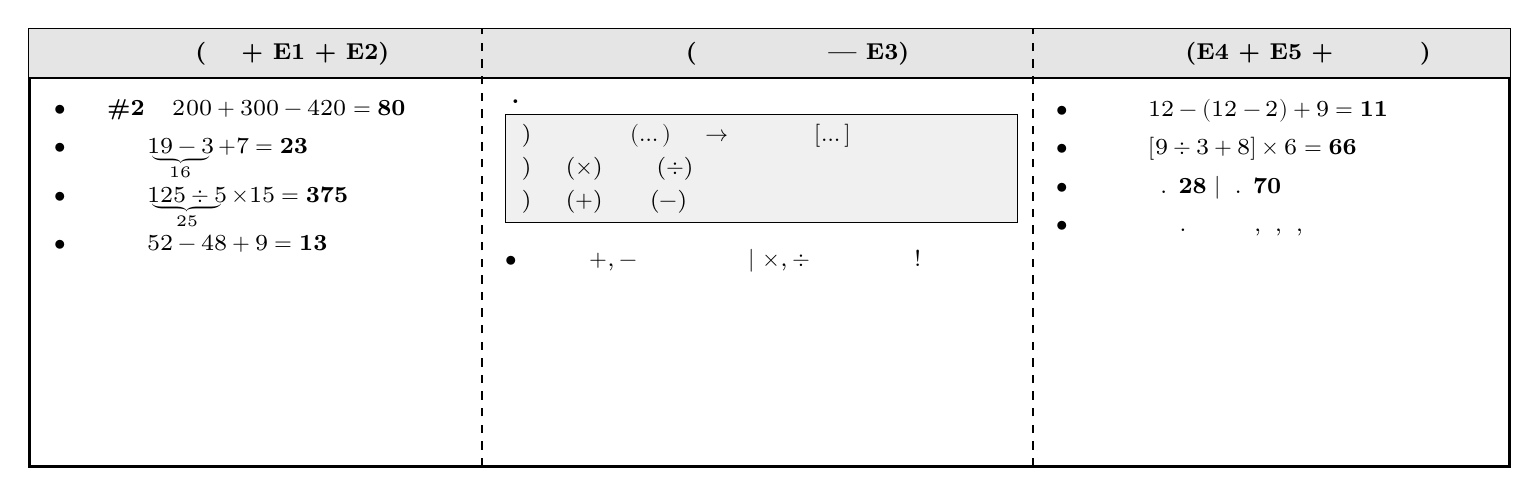
\begin{tikzpicture}[x=1cm, y=1cm, every node/.style={font=\fontsize{8.3pt}{11.8pt}\selectfont, text=black}]
  \draw[black, line width=1.1pt] (0,0) rectangle (18.8,5.55);
  \fill[gray!20] (0,4.93) rectangle (18.8,5.55);
  \draw[black, line width=0.7pt] (0,4.93) -- (18.8,4.93);
  \draw[black, dashed, line width=0.7pt] (5.75,0) -- (5.75,5.55);
  \draw[black, dashed, line width=0.7pt] (12.75,0) -- (12.75,5.55);

  \node at (2.875,5.24) {\textbf{ផ្នែកឆ្វេង (កំណែ + \en{E1} + \en{E2})}};
  \node at (9.25,5.24) {\textbf{ផ្នែកកណ្ដាល (ខ្លឹមសារគោលរក្សាទុក — \en{E3})}};
  \node at (15.775,5.24) {\textbf{ផ្នែកស្ដាំ (\en{E4} + \en{E5} + កិច្ចការផ្ទះ)}};

  % Left
  \node[anchor=north west, text width=5.30cm] at (0.20,4.78) {%
    $\bullet$ \textbf{កំណែ \#2 ក៖} $200+300-420=\mathbf{80}$\\[2pt]
    $\bullet$ \textbf{ឧទាហរណ៍ ១៖} $\underbrace{19-3}_{16}+7 = \mathbf{23}$\\[2pt]
    $\bullet$ \textbf{ឧទាហរណ៍ ៤៖} $\underbrace{125\div 5}_{25}\times 15 = \mathbf{375}$\\[2pt]
    $\bullet$ \textbf{ឧទាហរណ៍ ៥៖} $52 - 48 + 9 = \mathbf{13}$
  };

  % Center
  \node[anchor=north west, text width=6.65cm] at (5.92,4.78) {%
    {\muol\fontsize{8.5pt}{12pt}\selectfont ៦\enbf{.} លំដាប់នៃប្រមាណវិធីលើចំនួនគត់}\\[3pt]
    \tikz\node[draw=black, fill=gray!12, inner sep=3.5pt, text width=6.25cm]{%
      ១) ក្នុងវង់ក្រចក $(\dots)$ មុន $\to$ ក្នុងដង្កៀប $[\dots]$\\
      ២) គុណ ($\times$) និងចែក ($\div$) ពីឆ្វេងទៅស្ដាំ\\
      ៣) បូក ($+$) និងដក ($-$) ពីឆ្វេងទៅស្ដាំ
    };\\[4pt]
    $\bullet$ \textbf{ប្រយ័ត្ន៖} $+, -$ ស្មើអាទិភាពគ្នា $\mid$ $\times, \div$ ស្មើអាទិភាពគ្នា!
  };

  % Right
  \node[anchor=north west, text width=5.65cm] at (12.92,4.78) {%
    $\bullet$ \textbf{ឧទាហរណ៍ ៦៖} $12-(12-2)+9 = \mathbf{11}$\\[2pt]
    $\bullet$ \textbf{ឧទាហរណ៍ ៧៖} $[9\div 3+8]\times 6 = \mathbf{66}$\\[2pt]
    $\bullet$ \textbf{ប្រតិបត្តិ៖} ក. $\mathbf{28}$ $\mid$ ខ. $\mathbf{70}$\\[2pt]
    $\bullet$ \textbf{កិច្ចការផ្ទះ៖} ទំ.១៤ លេខ ២ ខ, គ, ឃ, ង
  };
\end{tikzpicture}
\end{center}

\vfill
\secstrip{២. ចម្លើយផ្ទៀងផ្ទាត់រហ័សសម្រាប់សន្លឹកកិច្ចការសិស្ស \enbf{(}ទំព័រ ១ និង ទំព័រ ២\enbf{)}}{\en{Answer Key}}

\begin{tcolorbox}[
  enhanced, sharp corners, colback=white, colframe=black,
  boxrule=0.8pt, boxsep=2.5pt, top=4.5pt, bottom=4.5pt, left=6pt, right=6pt
]
  \fontsize{9.0pt}{13.5pt}\selectfont
  $\bullet$ \textbf{ផ្នែក \en{E1}៖} \textbf{សិស្ស ខ} ត្រឹមត្រូវ ($23$) ចម្លើយខុសគ្នា ($9 \ne 23$) ត្រូវធ្វើពី\textbf{ឆ្វេងទៅស្ដាំ} ។\\[2pt]
  $\bullet$ \textbf{ផ្នែក \en{E2}៖} \textbf{សកម្មភាព ១៖} ឧ.២ $= 10+10-14 = 20-14 = \mathbf{6}$; ឧ.៣ $= 72\div 4 = \mathbf{18}$; ឧ.៤ $= 25\times 15 = \mathbf{375}$ ។ \textbf{សកម្មភាព ២៖} ឧ.៥ $= 52 - 48 + 3\times 3 = 52 - 48 + 9 = 4 + 9 = \mathbf{13}$ ។\\[2pt]
  $\bullet$ \textbf{ផ្នែក \en{E4}៖} ឧ.៦ $= 12-(12-2)+9 = 12-10+9 = 2+9 = \mathbf{11}$; ឧ.៧ $= [9\div 3+8]\times 6 = [3+8]\times 6 = 11\times 6 = \mathbf{66}$ ។ \en{EIA}៖ $12$ និង $4$ ។\\[2pt]
  $\bullet$ \textbf{ផ្នែក \en{E5}៖} \textbf{១) ប្រតិបត្តិ៖} ក. $8\times 4 - 12\div 3 = 32 - 4 = \mathbf{28}$; ខ. $[20\div 5 + 6]\times 7 = [4+6]\times 7 = \mathbf{70}$ ។ \textbf{២) បិទ \en{E1}៖} សិស្ស ខ ($23$) ។ \textbf{៣) វិនិច្ឆ័យ \en{A--D}៖} \textbf{ជម្រើស \en{C}} ($15$) ។ \textbf{៤) សំបុត្រចេញ៖} $24\div 6 + 15 = 4 + 15 = \mathbf{19}$ ។
\end{tcolorbox}

\vfill
\secstrip{៣. ចម្លើយលម្អិតនៃកិច្ចការផ្ទះ \enbf{(}សៀវភៅគោល ទំ.១៤ លេខ ២ ខ, គ, ឃ, ង\enbf{)}}{សៀវភៅគោល ទំ.១៤}

\begin{tcolorbox}[
  enhanced, sharp corners, colback=white, colframe=black,
  boxrule=0.8pt, boxsep=2.5pt, top=4.5pt, bottom=4.5pt, left=6pt, right=6pt
]
  \fontsize{8.8pt}{13.1pt}\selectfont
  $\bullet$ \textbf{ខ.} $(57 + 43 - 35) \times 20 + 360 = 65 \times 20 + 360 = 1\,300 + 360 = \mathbf{1\,660}$ ។ \quad
  $\bullet$ \textbf{គ.} $7 + 30 \div 5 - 13 = 7 + 6 - 13 = \mathbf{0}$ ។\\[2pt]
  $\bullet$ \textbf{ឃ.} $[60 + 9 - 24 \div 6] \times 2 = [69 - 4] \times 2 = 65 \times 2 = \mathbf{130}$ ។\\[2pt]
  $\bullet$ \textbf{ង.} $75 - 19 + 15\times 7 + 27\div 9\times 7 - 15 + 42 = 75 - 19 + 105 + 21 - 15 + 42 = 56 + 105 + 21 - 15 + 42 = \mathbf{209}$ ។
\end{tcolorbox}

\vfill
\secstrip{៤. ចំណុចប្រុងប្រយ័ត្នគរុកោសល្យសម្រាប់គ្រូ \enbf{(}ការយល់ច្រឡំសំខាន់ៗរបស់សិស្ស\enbf{)}}{\en{Pedagogical Watchlist}}

\begin{tcolorbox}[
  enhanced, sharp corners, colback=panelgray, colframe=black,
  boxrule=0.85pt, boxsep=2.5pt, top=4.5pt, bottom=4.5pt, left=6pt, right=6pt
]
  \fontsize{8.7pt}{12.9pt}\selectfont
  $\bullet$ \textbf{អន្ទាក់ «បូកមុនដក / គុណមុនចែក» (\en{Glidden, 2008})៖} បំបែកការយល់ច្រឡំនេះដោយបង្ហាញឧទាហរណ៍ ១ ($19-3+7=23$) និងឧទាហរណ៍ ៤ ($125\div 5\times 15 = 375$) ថា $(+,-)$ និង $(\times,\div)$ ត្រូវធ្វើពីឆ្វេងទៅស្ដាំជានិច្ច ។\\[2pt]
  $\bullet$ \textbf{កំណត់សម្គាល់អក្ខរាវិរុទ្ធក្នុងសៀវភៅគោលទំ.១០៖} ប្រអប់ជាទូទៅក្រោមឧទាហរណ៍ ៧ បោះពុម្ពថា \emph{«តង្កៀប»} សូមគ្រូណែនាំអក្ខរាវិរុទ្ធផ្លូវការថា \textbf{«ដង្កៀប»} ($[\dots]$) ។
\end{tcolorbox}

\end{document}
